\documentclass[10pt,a4paper]{amsart}
\usepackage[margin=19mm]{geometry}
\usepackage{amsmath,amssymb,mathtools}
\usepackage[scr=rsfs,cal=euler]{mathalfa}
\usepackage{xfrac}
\usepackage[unicode,hidelinks,bookmarks=false]{hyperref}
\newcommand{\ie}{i.e.\ }
\newcommand{\cf}{cf.\ }
\newcommand{\resp}{respectively\ }
\newcommand{\Subsection}{\subsection}
\providecommand{\nobreakdash}{\nobreak\hbox{-}}
\setlength{\emergencystretch}{2em}
\multlinegap0pt
\usepackage{tikz}
\usepackage{amssymb}
\usepackage{mathtools}
\usepackage{xcolor}
\newtheorem{lemma}{Lemma}
\newcommand{\calP}{\mathcal{P}}
\newcommand{\exx}{\mathrm{ex}}
\newcommand{\highlight}[1]{\colorbox{gray!15}{\small{#1}}}
\title{Orderings on $k$-Markov Numbers}
\author{Esther Banaian}
\date{Source: arXiv:2512.04026v2 (CC BY 4.0)}
\begin{document}
\maketitle

\noindent\emph{Source and licence.} Orderings on $k$-Markov Numbers. Version arXiv:2512.04026v2 (CC BY 4.0), distributed by arXiv under the Creative Commons Attribution 4.0 International licence, http://creativecommons.org/licenses/by/4.0/, as recorded in the arXiv licence metadata for this exact version and shown on the abstract page https://arxiv.org/abs/2512.04026v2. Full licence notice: \texttt{licenses/arxiv-2512.04026-CC-BY-4.0.txt}.\par\smallskip

\noindent\textit{Editorial scope.} Counted unit: the article's lemma lem:SelfIntNotMinimal (source0.tex lines 1150--1152). The article's complete original proof of it is delivered with it (source0.tex lines 1154--1223, one \texttt{proof} environment of 70 lines). No mathematics is written, repaired or re-derived: the statement and the proof are the article's own lines, in the article's own notation, and no retained line is substituted or re-flowed.  No further source-local context is needed: every cross-reference of every retained line resolves inside the two delivered spans.  Nothing was omitted from any retained span, so the package carries no omission record.  No retained line contains a citation, so the wrapper carries no bibliography and no bibliography entry.  The retained lines contain the article's own diagram code, which the wrapper typesets with the standard tikz packages; no image file is delivered and the package declares no asset dependency.  Editorial formatting only, in addition: an AMS \texttt{amsart} preamble that restates the article's own declarations and macros used by the retained lines, namely the environments \texttt{lemma} on separate counters, together with the standard packages those lines need.  The retained environments print in this document as Lemma 1 in order of appearance, whereas the article prints the same items with the numbering of its own full document.  The complete native source of the article as distributed in the arXiv e-print for this exact version is bundled unchanged as \texttt{sources/190303/source0.tex}.
\begin{lemma}\label{lem:SelfIntNotMinimal}
If $\gamma$ is an arc with endpoints $A,B$ which has a non-contractible self-intersection, then $\ell_k(\gamma) > \vert AB \vert_k$.
\end{lemma}

\begin{proof}
The claim is trivial if $A = B$, since $\vert AA \vert_k = 0$, so we assume $A$ and $B$ are distinct. Let $\gamma$ be an arc with a point of self-intersection. Call this point $C$. Since $\gamma$ visits $C$ twice, we can divide $\gamma$ into three curves $\gamma_1,\gamma_2,\gamma_3$ consisting of the portion of $\gamma$ before the first time it passes through $C$, the portion between its two instances of passing through $C$, and the portion after the last instance.  In particular, giving each $\gamma_i$ the orientation inherited from $\gamma$, $\gamma_1$ starts at $A$ and $\gamma_3$ ends at $B$.  Let $\gamma'$ be the result of concatenating $\gamma_1$ and $\gamma_3$ and removing unnecessary intersections of the resulting arc with $\mathcal{L}$. Do this in such a way to preserve the location of the intersection points of all unaffected crossings between the $\gamma_1$ and $\mathcal{L}$ and similarly for $\gamma_3$. 

Removing the unnecessary intersections is akin to pulling $C$, the point of self-intersection, back to an extreme triangle. Assume first that $C$ cannot be pulled back to the first or last triangle which $\gamma$ passes through. Then, the configuration of $\gamma$ and $\gamma'$ is as below. 

\begin{center}
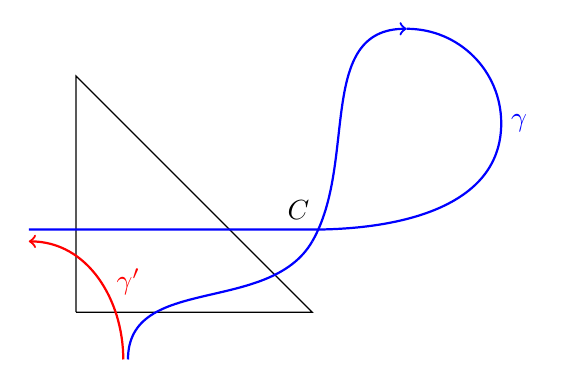
\begin{tikzpicture}[scale = 3]
\draw(0,0) to  (1,0) to (0,1) to (0,0); 
\draw[red, thick,<-] (-0.2,0.3) to [out = 0, in = 90] (0.2,-0.2);
\draw[blue, thick,] (-0.2,0.35) to [out = 0, in = 180] (1,0.35) to [out = 0, in = -90] (1.8,0.8) to [out = 90, in = 0] (1.4,1.2);
\draw[blue,thick,<-] (1.4,1.2)to [out = 180, in = 60] (1,0.3);
\draw[blue,thick] (1,0.3) to [out = 240, in = 90] (0.22,-0.2);
\node[right, blue] at (1.8,0.8){$\gamma$};
\node[red, right] at (0.13,0.13){$\gamma'$};
\node[above, xshift = -5pt] at (1,0.35){$C$};
\end{tikzpicture}   
\end{center}


We will show $\ell_k(\gamma) > \ell_k(\gamma')$ by exhibiting an injection from $J(\calP_{\gamma'}^\exx)$ to $J(\calP_\gamma^\exx)$ which has a nonempty cokernel. Let $h = \vert \calP_\gamma^\exx \vert$. By our construction of $\gamma'$, there are values $u < v$ such that $\calP_{\gamma'}^\exx$ is the result of taking the induced subposet on $\calP_\gamma[1,u] \cup \calP_\gamma[v,h]$ and adding a relation between $\calP_\gamma(u)$ and $\calP_\gamma(v)$. If $\gamma$ has the orientation as above, inducing an orientation on $\gamma'$ as well, then the posets $\calP_\gamma$ and $\calP_{\gamma'}$ are as below. By abuse of notation, we will retain the chronological labeling from $\calP_\gamma^\exx$ when referencing elements of $\calP_{\gamma'}^\exx$. There are two cases to consider; first, assume that $\calP_\gamma(u+1)$ and $\calP_\gamma(v-1)$ are incomparable. 
%If $\gamma'$ and $\gamma$ are as above, then up to orientation, $\calP_\gamma(u)$ is labeled by $z$ and $\calP_\gamma(v)$ is labeled by $x$. With this choice of orientation, we add to $\calP_{\gamma'}$ the relation $\calP_\gamma(u) \succ \calP_\gamma(v)$. Moreover, $\calP^\exx_\gamma(u+1)$ and $\calP^\exx_\gamma(v-1)$ are both labeled by $y$. 



\begin{center}
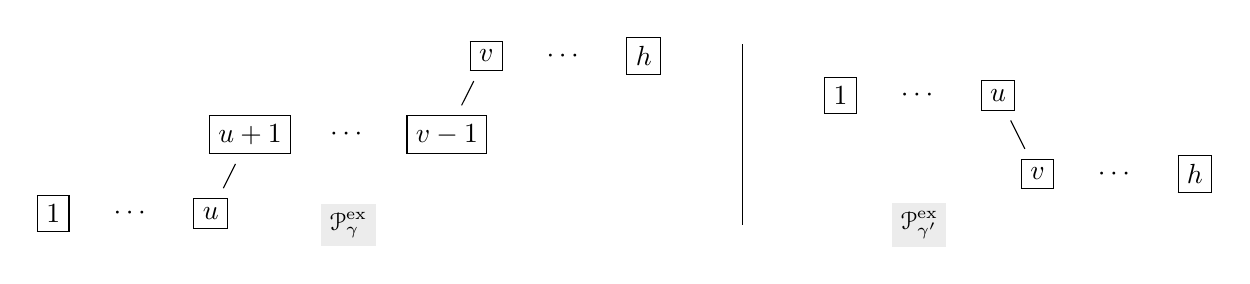
\begin{tikzpicture}
\node[] at (0.5,0) {$\boxed{1}$};
\node[] at (1.5,0){$\cdots$};
\node(s) at (2.5,0){$\boxed{u}$};
\node(s+1) at (3,1){$\boxed{u+1}$};
\node[] at (4.25,1){$\cdots$};
\node(t-1) at (5.5,1){$\boxed{v-1}$};
\node(t) at (6,2){$\boxed{v}$};
\node[] at (7,2){$\cdots$};
\node[] at (8,2) {$\boxed{h}$};
\draw(s)--(s+1);
\draw(t-1)--(t);
\node[] at (4.25,-0.15){\highlight{$\calP^\exx_\gamma$}};
\draw(9.25,2.15) -- (9.25,-0.15);
\node[] at (10.5,1.5) {$\boxed{1}$};
\node[] at (11.5,1.5){$\cdots$};
\node(s') at (12.5,1.5){$\boxed{u}$};
\node(t') at (13,0.5){$\boxed{v}$};
\node[] at (14,0.5){$\cdots$};
\node[] at (15,0.5) {$\boxed{h}$};
\node[] at (11.5,-0.15){\highlight{$\calP^\exx_{\gamma'}$}};
\draw(s')--(t');
\end{tikzpicture}
\end{center}


 Every order ideal $I'$ of $\calP_{\gamma'}^\exx$ can naturally be viewed as an order ideal $I$ of $\calP_{\gamma}^\exx$ where we include the set $\langle \calP^\exx_{\gamma}(v-1)\rangle$ if $\calP^\exx_{\gamma}(v) \in I'$.Since we assumed  $\calP_\gamma(u+1)$ and $\calP_\gamma(v-1)$, this correspondence of sending $I' \in J(\calP_{\gamma'}^\exx)$ to $I \in J(\calP_{\gamma}^\exx)$ is a non-surjective injection, implying $\vert J(\calP_{\gamma'}^\exx) \vert < \vert J(\calP_{\gamma}^\exx) \vert$.

 Now, suppose that $\calP_\gamma(u+1)$ and $\calP_\gamma(v-1)$ are comparable. This only occurs if the self-intersection comes from $\gamma$ winding around a single integral point. This winding introduces a chain in $\calP_\gamma$. By either considering order ideals which contain this entire chain or which do not intersect this chain, one can similarly build an injection from $J(\calP_{\gamma'}^\exx)$ to $J(\calP_\gamma^\exx)$.

Finally, suppose that $C$ can be pulled back to the first triangle with $\gamma$ passes through. 

\begin{center}
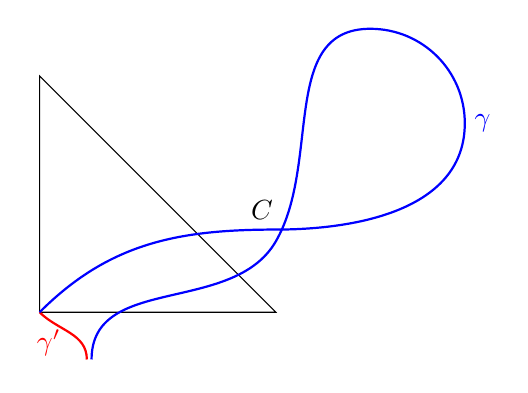
\begin{tikzpicture}[scale = 3]
\draw(0,0) to (1,0) to (0,1) to  (0,0); 
\draw[red, thick] (0,0) to [out = -45, in = 90] (0.2,-0.2);
\draw[blue, thick] (0,0) to [out = 45, in = 180] (1,0.35) to [out = 0, in = -90] (1.8,0.8) to [out = 90, in = 0] (1.4,1.2) to [out = 180, in = 60] (1,0.3) to [out = 240, in = 90] (0.22,-0.2);
\node[right, blue] at (1.8,0.8){$\gamma$};
\node[red, left] at (0.13,-0.13){$\gamma'$};
\node[above, xshift = -5pt] at (1,0.35){$C$};
\end{tikzpicture}   
\end{center}

In this case, $\calP_{\gamma'}^\exx$ is of the form $\calP_{\gamma}^\exx[v,h]$ where again $h$ denotes the cardinality of $\calP_{\gamma}^\exx$. Our set-up here implies that there exists at least one value $i < v$ such that $\calP_{\gamma}^\exx(i)$ and $\calP_{\gamma}^\exx(v)$ are incomparable, and therefore it is clear that $\vert J(\calP_{\gamma'}^\exx) \vert < \vert J(\calP_{\gamma}^\exx) \vert$.
\end{proof}

\end{document}
